\documentclass{beamer}
\usetheme{Boadilla}
\usecolortheme{sidebartab}

\usepackage{hyperref}
\usepackage{showexpl} 
\usepackage{graphicx}
\usepackage{color}
\usepackage{siunitx}
\usepackage[version=3]{mhchem}
\usepackage{chemfig}
\usepackage{changes}

\beamertemplatenavigationsymbolsempty
\setbeamertemplate{footline}{}
\setbeamertemplate{bibliography item}{\insertbiblabel}

\lstloadlanguages{[LaTeX]Tex} 
\lstset{% 
     basicstyle=\ttfamily\large, 
     commentstyle=\itshape\ttfamily, 
     showspaces=false, 
     showstringspaces=false, 
     breaklines=true, 
     breakautoindent=false, 
     captionpos=t,
     explpreset={numbers=none},
     pos=b
} 

\title{Research Data and Data Management Planning}
\author{Markus Stocker}
\date{September 12, 2017}

\begin{document}

\maketitle

\begin{frame}
  \frametitle{Outline}
  
  \begin{itemize}
  \item What are research data
  \item Research data lifecycle
  \item Data types, formats, models and standards
  \item Metadata
  \item Data management, plans and planning tools
  \end{itemize}
\end{frame}

% Datum is ultimately reducible to a lack of uniformity, between signals, symbols
% Data depend on the occurrence of differences
% Defined as x being distinct from y
% Where x, y are uninterpreted (typed) variables
% Variable is a symbol that acts as a placeholder for an unknown (or changeable) referent
% Referent: the thing in the world that the symbol denotes (or stands) for
{
	\usebackgroundtemplate{ %
		\begin{tikzpicture}[remember picture, overlay]%
		\node at (current page.center) {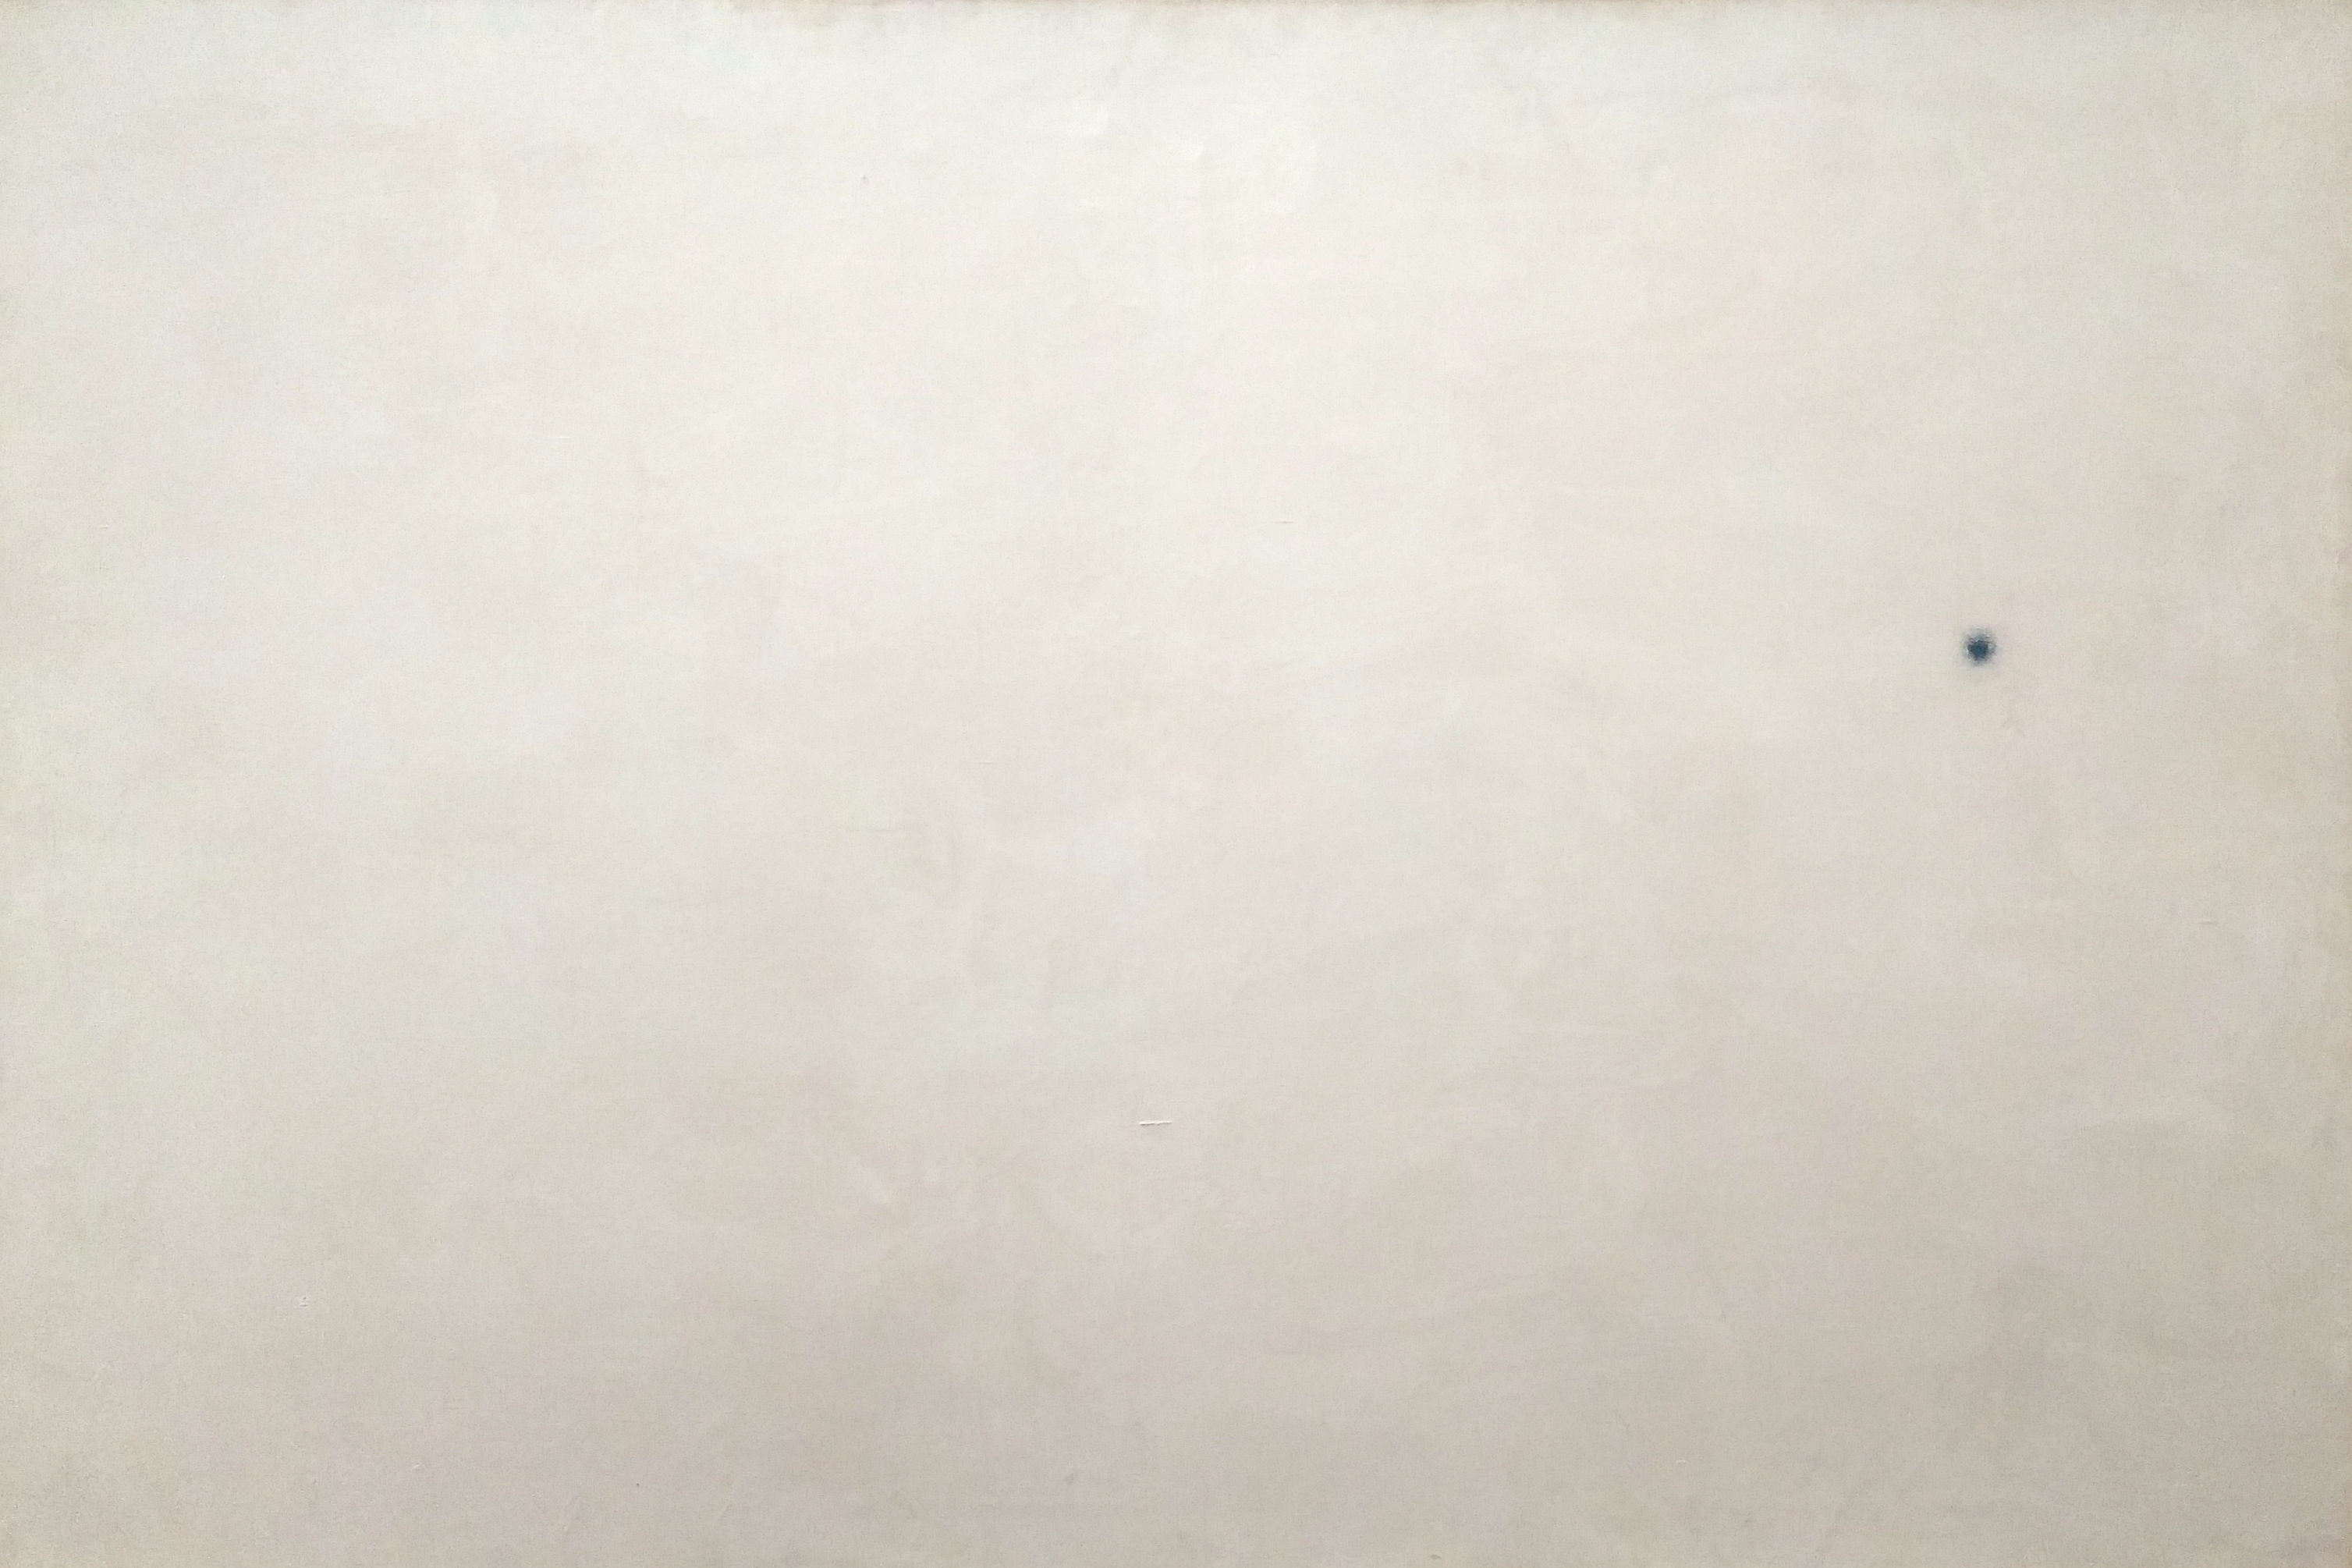
\includegraphics[height=\paperheight]{graphics/joan-miro-landscape-1968.jpg}};%
		\end{tikzpicture}%
	}%
	\setbeamertemplate{navigation symbols}{}
	\begin{frame}[plain]
	\end{frame}
}

\begin{frame}
  \frametitle{Data}
  
  \begin{itemize}
  \item 
  \end{itemize}
\end{frame}

\begin{frame}
  \frametitle{Research data}
  
  \begin{itemize}
  \item 
  \end{itemize}
\end{frame}

\begin{frame}
  \frametitle{Research data lifecycle}
  
  \begin{itemize}
  \item 
  \end{itemize}
\end{frame}

\begin{frame}
  \frametitle{Data types}
  
  \begin{itemize}
  \item 
  \end{itemize}
\end{frame}

\begin{frame}
  \frametitle{Data formats}
  
  \begin{itemize}
  \item 
  \end{itemize}
\end{frame}

\begin{frame}
  \frametitle{Data models}
  
  \begin{itemize}
  \item 
  \end{itemize}
\end{frame}

\begin{frame}
  \frametitle{Standards}
  
  \begin{itemize}
  \item 
  \end{itemize}
\end{frame}

\begin{frame}
  \frametitle{Metadata}
  
  \begin{itemize}
  \item 
  \end{itemize}
\end{frame}

\begin{frame}
  \frametitle{Data management}
  
  \begin{itemize}
  \item 
  \end{itemize}
\end{frame}

\begin{frame}
  \frametitle{Planning data management}
  
  \begin{itemize}
  \item 
  \end{itemize}
\end{frame}

\begin{frame}
  \frametitle{Tools for data management planning}
  
  \begin{itemize}
  \item 
  \end{itemize}
\end{frame}

\begin{frame}
  \frametitle{Take aways}
  
\end{frame}

\begin{frame}
  \frametitle{References}
  \tiny
  \bibliographystyle{plain} 
  \bibliography{../../../../../bibliography/bibliography}
  
  Slide 3: Joan Mir{\'o} (1968). Landscape. Acrylic on canvas. Fundaci{\'o}n Joan Mir{\'o}, Barcelona. \url{https://www.fmirobcn.org/en/colection/catalog-works/5442/p-landscape-p}
\end{frame}

\end{document}
